\question[25] % DRG

%% Use this if you have both Spanish and English versions
%% \ifspanish
%% % Here the Spanish version
%% \else
%% % Here the English version
%% \fi

Consider a detection problem with three hypothesis ($H \in\{0,1,2\}$), observation $\mathbf{X} = (X_1, X_2)^T \in \mathbb{R}^2$ and likelihoods
\begin{align*}
p_{\mathbf{X}|H}(\mathbf{x}|0) &= \frac{1}{\pi}, \qquad  x_1^2 + x_2^2 < 1,                \\
p_{\mathbf{X}|H}(\mathbf{x}|1) &= \frac{1}{4},   \qquad  0 < x_1 < 2,  \quad 0 < x_2 < 2,   \\
p_{\mathbf{X}|H}(\mathbf{x}|2) &= 1,             \qquad  1 < x_1 < 2,  \quad  1 < x_2 < 2,   \\
\end{align*}
The a priori probabilities are $P_H(0) = 1/8$, $P_H(1) = 1/2$, and $P_H(2) = 3/8$.

Find:
\begin{parts}
\part[10]
The decision regions of the detector that minimizes the probability of error.

\begin{solution}
   The detector that minimizes the probability of error is the maximum a posteriori detector, which is given by
   \begin{equation*}
      d = \arg \mathop{\operatorname{max}}_{h} P_{H|\mathbf{X}}(h|\mathbf{x}),
    \end{equation*}
    and can be rewritten as
   \begin{equation*}
      d = \arg \mathop{\operatorname{max}}_{h} p_{\mathbf{X}|H}(\mathbf{x}|h) P_H(h).
    \end{equation*}
    Hence, the decision regions are
  \begin{equation*}
    \mathcal{X}_d = \{\mathbf{x} | d = \arg \mathop{\operatorname{max}}_{h} p_{\mathbf{X}|H}(\mathbf{x}|h) P_H(h)\}.
  \end{equation*}
  To compute these decision regions, it is convenient to plot the supports of the likelihoods as shown in the next figure (each colored line corresponds to the support boundary)
  \begin{center}
	        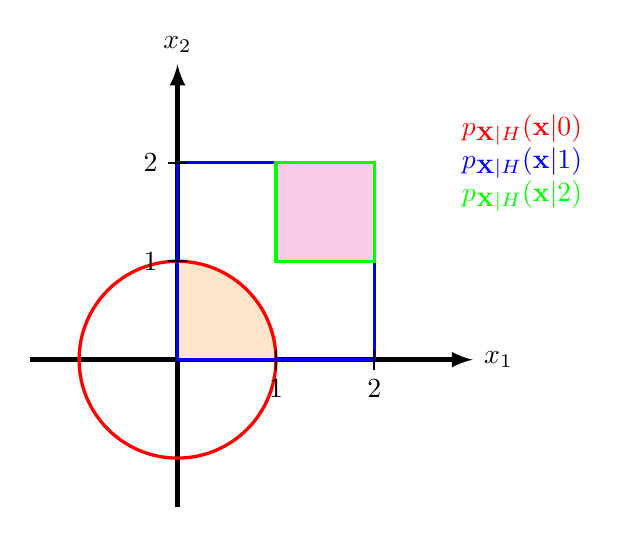
\begin{tikzpicture}[scale=1.25,cap=butt]
  \usetikzlibrary{arrows} % LATEX and plain TEX when using TikZ
  
  % Axis
  \draw[-latex,black,ultra thick] (-1.5,0) -- (3,0) node[right,black] {$x_1$};
  \draw[-latex,black,ultra thick] (0,-1.5) -- (0,3) node[above,black] {$x_2$};
  
  % Supports
  \fill[fill=orange!20] (0,0) -- (1,0) arc[start angle=0, end angle=90, radius=1] -- cycle;
  \fill[fill=magenta!20] (1,1) -- (2,1) -- (2,2) -- (1,2) -- cycle;
  \draw[color=red, very thick](0,0) circle (1);
  \draw[blue, very thick] (0,0) rectangle (2,2);
  \draw[green, very thick] (1,1) rectangle (2,2);
  
  % Ticks
  \draw[black,thick] (2,-0.1) node[below,black] {$2$} -- (2,0.1);
  \draw[black,thick] (1,-0.1) node[below,black] {$1$} -- (1,0.1);
  \draw[black,thick] (-0.1,2) node[left,black] {$2$} -- (0.1,2);
  \draw[black,thick] (-0.1,1) node[left,black] {$1$} -- (0.1,1);
  
    % Legend
  \node[draw,align=left,draw=none] at (3.5,2) {\textcolor{red}{$p_{\mathbf{X}|H}(\mathbf{x}|0)$} \\ \textcolor{blue}{$p_{\mathbf{X}|H}(\mathbf{x}|1)$} \\ \textcolor{green}{$p_{\mathbf{X}|H}(\mathbf{x}|2)$}};
  
\end{tikzpicture}
\end{center}
From this plot, we can see that the supports of the likelihoods only overlap in two regions, which are shaded. Then, we only need to see which $p_{X|H}(x|h) P_H(h)$ is larger in these region. In the orange-shaded area, it is easy to see that
\begin{equation*}
p_{X|H}(x|0) P_H(0) = \frac{1}{\pi} \cdot \frac{1}{8} < p_{X|H}(x|1) P_H(1) = \frac{1}{4} \cdot \frac{1}{2}, 
\end{equation*}
and, therefore, in this region we should decide $D = 1$. In the magenta-shaded area, we have
\begin{equation*}
p_{X|H}(x|1) P_H(1) = \frac{1}{4} \cdot \frac{1}{2} < p_{X|H}(x|2) P_H(2) = 1 \cdot \frac{3}{8},
\end{equation*}
which implies that in this region we should decide $D = 2$. Hence, the decision regions are
\begin{align*}
\mathcal{X}_0 &= \{(x_1, x_2)^T \mid x_1^2 + x_2^2 < 1, x_1 \leq 0\} \cup \{(x_1, x_2)^T \mid x_1^2 + x_2^2 < 1, x_1 > 0, x_2 \leq 0 \}, \\
\mathcal{X}_1 &= \{(x_1, x_2)^T \mid 0 < x_1 \leq 1, 0 < x_2 < 2 \} \cup \{(x_1, x_2)^T \mid 1 < x_1 < 2, 0 < x_2 \leq 1 \}  \\
\mathcal{X}_2 &= \{(x_1, x_2)^T \mid 1 < x_1 < 2, 1 < x_2 < 2 \},
\end{align*}
which are the shaded areas shown in the following figure
  \begin{center}
	        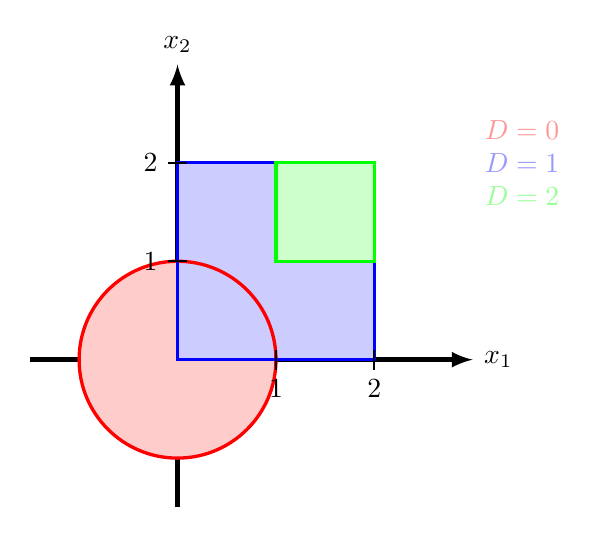
\begin{tikzpicture}[scale=1.25,cap=butt]
  \usetikzlibrary{arrows} % LATEX and plain TEX when using TikZ
  
  % Axis
  \draw[-latex,black,ultra thick] (-1.5,0) -- (3,0) node[right,black] {$x_1$};
  \draw[-latex,black,ultra thick] (0,-1.5) -- (0,3) node[above,black] {$x_2$};
  
  % Supports
  \fill[fill=red!20] (0,0) -- (0,1) arc[start angle=90, end angle=360, radius=1] -- cycle;
  \fill[fill=blue!20] (1,1) -- (2,1) -- (2,0) -- (0,0) -- (0,2) -- (1,2) -- cycle;
  \fill[fill=green!20] (1,1) -- (2,1) -- (2,2) -- (1,2) -- cycle;
  \draw[color=red, very thick](0,0) circle (1);
  \draw[blue, very thick] (0,0) rectangle (2,2);
  \draw[green, very thick] (1,1) rectangle (2,2);
  
  % Ticks
  \draw[black,thick] (2,-0.1) node[below,black] {$2$} -- (2,0.1);
  \draw[black,thick] (1,-0.1) node[below,black] {$1$} -- (1,0.1);
  \draw[black,thick] (-0.1,2) node[left,black] {$2$} -- (0.1,2);
  \draw[black,thick] (-0.1,1) node[left,black] {$1$} -- (0.1,1);
  
  % Legend
  \node[draw,align=left,draw=none] at (3.5,2) {\textcolor{red!40}{$D = 0$} \\ \textcolor{blue!40}{$D = 1$} \\ \textcolor{green!40}{$D = 2$}};
  
\end{tikzpicture}
	\end{center}
        
  
\end{solution}

\part[10]
The conditional probability of correct decision of the derived detector under $H = 0$, $P(D = 0 | H = 0)$.
  
\begin{solution}
  The requested probability is
  \begin{equation*}
    P(D = 0 | H = 0) = \int_{\mathcal{X}_0} p_{\mathbf{X}|H}(\mathbf{x}|0) d \mathbf{x}.
  \end{equation*}
  That is, we need to integrate the constant $p_{\mathbf{X}|H}(\mathbf{x}|0) = 1/\pi$ in the region $\mathcal{X}_0$. Since we know that $p_{\mathbf{X}|H}(\mathbf{x}|0) = 1/\pi$ integrates to $1$ in the region $\{(x_1, x_2)^T \mid x_1^2 + x_2^2 < 1\}$, and we are leaving out one quarter of that region, $P(D = 0 | H = 0)$ becomes
  \begin{equation*}
    P(D = 0 | H = 0) = \frac{3}{4}.
  \end{equation*}
  
\end{solution}
  
\end{parts}

